\chapter{Background}
\lhead{\emph{Background}}

\section{Introduction to the History of Computer Vision}
\label{sec:intro}


Computer vision is a relatively old field in computer science. The subject itself has been around since the 1960s, but it is only recently that it has been possible to build useful computer systems ideas from computer vision \citep {cv}.
The birthday of Computer Vision is considered the summer of 1966.  During that year a computer vision summer project was proposed in the MIT AI lab. The goal of the summer vision project was to use summer workers (students) effectively in the construction of a significant part of a visual system  \citep{papert}. It was thought that vision was a relatively easy field of AI and that a landmark in the development of pattern recognition could be achieved during the summer. The task, however, was a lot harder than previously expected and no significant computer vision problems were solved during that project.

During development of a computer vision, it was noticed that is very hard to recognise an object by describing the whole image. Pixel variation in images that are produced under different conditions is high. Therefore, important features have to be selected to make a picture more resistible to various variations. Later these selected features are used for detecting a particular object. In 1999 a new method for image feature generation called the Scale Invariant Feature Transform (SIFT) was proposed by \cite{sift}. These features are invariant to image scaling, translation, and rotation, and partially invariant to illumination changes. Because of that SIFT features performed much better than correlation-based template matching technique that was used before and could be seen as a major break point in computer vision.
 
Another method for detecting features in images was proposed by \cite{nakano2006object}. The authors of this paper state that since objects are composed of a combination of characteristic parts. A good object detector could be developed if local parts specialised for a detection target were derived automatically from the training samples. To do this, researchers used independent component analysis (ICA) which decomposed a signal into separate elementary signals. Then ICA vectors were applied to the candidate area, and their outputs were used in classification. Using this approach face detector algorithm used in Fujifilm camera with real-time face detection was created. It is considered to be a first commercial application that could run computer vision algorithms in real time. 
 
The important turning point in the development of computer vision field was a creation of the ImageNet dataset and the ImageNet Large Scale Visual Recognition Challenge in 2010. The challenge is a competition where research teams submit image classification models that classify and detect objects. The challenge is running annually since 2010. In 2010 the goal of the challenge was to estimate the content of photographs for the purpose of retrieval and automatic annotation using a subset of the large hand-labeled ImageNet dataset (10,000,000 labelled images depicting 10,000+ object categories) as the training set \citep{ImageNet}. Example images from the ImageNet which represent a pizza class can be seen in \autoref{fig:imgnet}.


Because of many images and categories, ImageNet is still a huge challenge for researchers who try to build classification models for the challenge.  ImageNet encourages improvement and innovation in computer vision techniques. In 2012 ImageNet competition was won by an approach that used convolutional neural networks- AlexNet \citep{alex}. Since then deep learning became a dominant method for an image classification. 


 \begin{figure}[h]
\centering
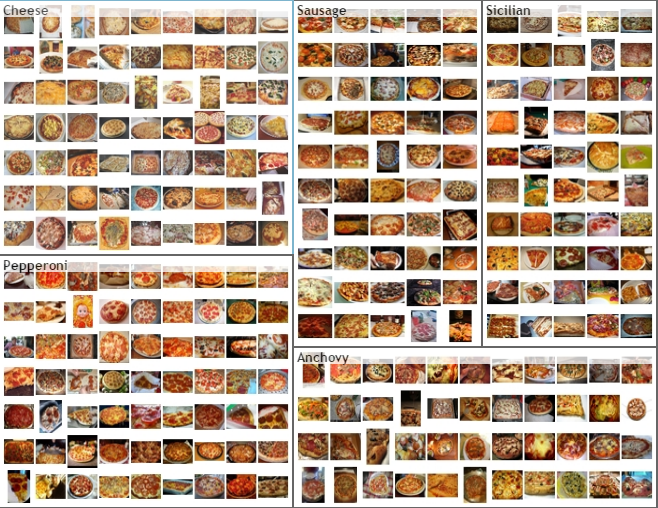
\includegraphics[width=10cm]{Figures/2/imgnet.PNG}
\caption{Example ImageNet Images of a Pizza Class }
\label{fig:imgnet}
\end{figure}


\section{Why is Computer Vision a Hard Problem?}
The true challenge to artificial intelligence proved to be solving the tasks that are easy for people to perform but hard for people to describe formally - problems that we solve intuitively, that feel automatic, like recognising objects in images \citep{Goodfellow-et-al-2017}.

A human can identify objects in images under all kinds of changes in illumination, viewpoint, scale, etc. In comparison, computer algorithms are very susceptible to all sorts of variations. Major variations in pictures were defined by \cite{231n} as:

\begin{enumerate}
\item Viewpoint variation. A single instance of an object can be oriented in many ways with respect to the camera.
\item Scale variation. Visual classes often exhibit variation in their size (size in the real world, not only in terms of their extent in the image).
\item Deformation. Many objects of interest are not rigid bodies and can be deformed in extreme ways.
\item Occlusion. The objects of interest can be occluded. Sometimes only a small portion of an object can be visible.
\item Illumination conditions. The effects of illumination are drastic on the pixel level.
\item Background clutter. The objects of interest may blend into their environment, making them hard to identify.
\item Intra-class variation. The classes of interest can often be relatively broad, such as a chair. There are many different types of these objects, each with their own appearance.
\end{enumerate}


 \begin{figure}[h]
\centering
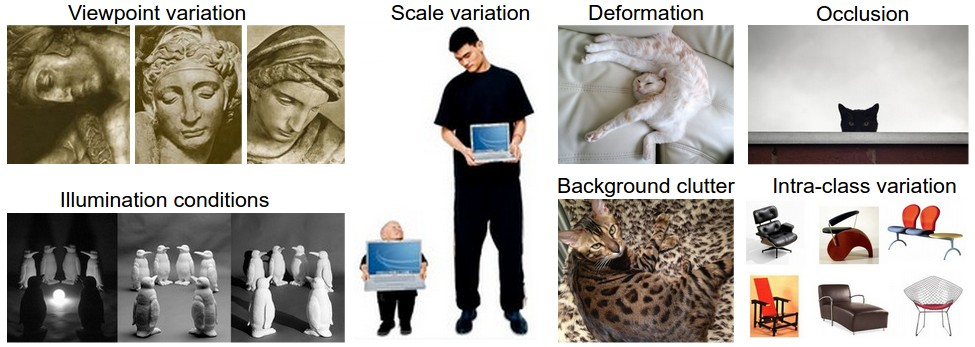
\includegraphics[width=14cm]{Figures/2/challenges.jpeg}
\caption{Example of Various Variations in Images \citep{231n}}
\label{fig:imgnet}
\end{figure}

The actual solution to the variation problem still has not been found. Currently,  either this issue is ignored, or algorithms that are partly resistant to variations are used.

\section{ Review of the  Study of an Automatic Food Image Segmentation }
A computer system that can be utilized for an image-based dietary assessment was described by \cite{chen2015saliency}. A wearable computer called eButton was used to capture the eating events. The eButton is a small chest camera that can be pinned on clothes. The camera can take pictures automatically at the rate of one image per second. Then, segmentation techniques are applied to segment food from a container. Finally, a person manually enters the food label to the application. The operational diagram of the eButton (\autoref{fig:1}) states that food volume measurement, nutrient database lookup, and calculation of calories are also performed by the device. However, these operations were not described in the paper. 

\begin{figure}[ht]
\centering
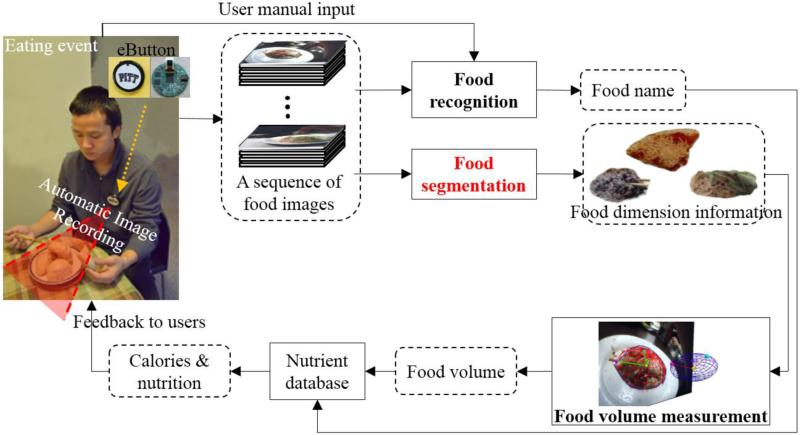
\includegraphics{Figures/segm_01.jpg}
\caption{Personal Dietary Assessment with eButton} from \citep{chen2015saliency} 
\label{fig:1}
\end{figure}

The main focus of the paper was a food segmentation from its container. Authors stated that major difficulties in automatic food segmentation are multiple food components in a container, coloured decorative patterns on plates and occlusion by other objects. The example images of these three difficulties are shown in \autoref{fig:2}.

\begin{figure}[ht]
\centering
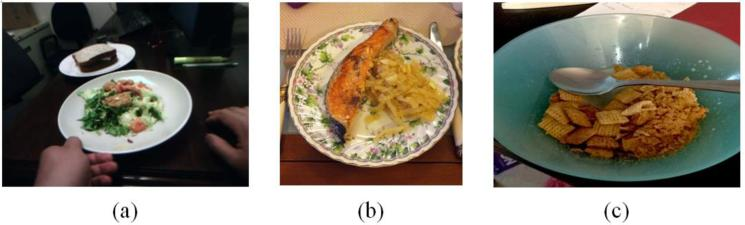
\includegraphics{Figures/segm_02.jpg}
\caption{Major Difficulties in Automatic Food Segmentation} from \citep{chen2015saliency}
\label{fig:2}
\end{figure}


Researchers approached an image segmentation in the two stages. Firstly, a food container was detected in an image by its shape convexity. Canny edge detector was used to obtain the edge information from a given image. Then, some squares at edge pixels were randomly selected \autoref{fig:3}. Then, squares not belonging to the container edge were discarded, and the area of the container was detected.

For segmenting food inside a plate, researchers used the color contrast between objects and surroundings, colour abundance and spatial arrangement. That allowed to recognise the areas in the image with one highly dominant colour. These three characteristics were then combined to segment food from a container.

The data set used to evaluate the segmentation approach in this research was combined from 30 eating events captured with eButton and 30 food images from the Jawbone database. Accuracy was measured by visually inspecting the quality of the segmentation and by comparing the image segmented by a computer to the pictures segmented by two research participants. The average error rate of the machine was  8.443 \pm\ 5.203 mm. 



\begin{figure}[ht]
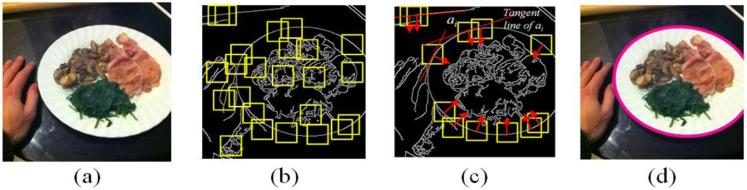
\includegraphics{Figures/2/segm_03.jpg}
\caption{Container Detection;  from \citep{chen2015saliency}}
\label{fig:3}
\end{figure}
To conclude, this study proved that food segmentation from images was possible. However, the dataset used to evaluate the segmentation approach was too small to make a general conclusion whether this approach is suitable for various kinds of food images.
The main limitation of the image segmentation by shape convexity is that in some cases food is served not in a round shaped container, for example take away food box or a lunch box. Some of the foods can also be eaten without using any container at all, for instance fruits and vegetables.

\iffalse
\section{Food-101 Mining Discriminative components with random forests}
This paper address the problem of automatically recognising pictured dishes. A novel method is proposed to mine discriminative parts using Random Forests, which allowed to mine for parts simultaneously for all classes and to share knowledge among them.
A dataset of 101 food categories, with 101’000 images, was created by the authors of the paper.  Random forest classification method produced an average accuracy of 50.76 percent.
\fi
\section{Survey of Applications for Counting Calories}

 It was decided to try currently available applications for calorie counting, to get a better understanding what are the input methods offered by them. To get applications keyword ``calorie counting" was entered into the search bar of the Google Play Store. The top 3 apps in the search results were downloaded and tested. These apps were MyFitnessPal, Nutracheck, and Lifesum.

MyfitnessPal is the most popular calorie-counting app on the Google Play Store. The app has over 50 million downloads on Google Play Store (\autoref{fig:mfp}). When the app is launched for the first time the user is required to sign up. After entering his email and password, the user has to complete a short survey about his goal, physical activity levels, gender, birthday, location, weight and height, desired weight and agree to the privacy policy and terms (\autoref{fig:mfp2}). After that, the app calculates target daily calorie intake. For entering food, user can scan the barcode of the food or use the text-based search. Food search and barcode scanning only work when a phone is connected to the Internet.  The database of food items is quite broad and includes products from many different restaurants. However,  adding a meal that was prepared by a user himself is complicated. Every ingredient of the dish must be searched and added separately.  The portion size has to be entered using weight measurements, for example,  grams. It is a significant disadvantage because it is often hard to estimate the weight of the meal.
 
\begin{figure}[ht]
\centering
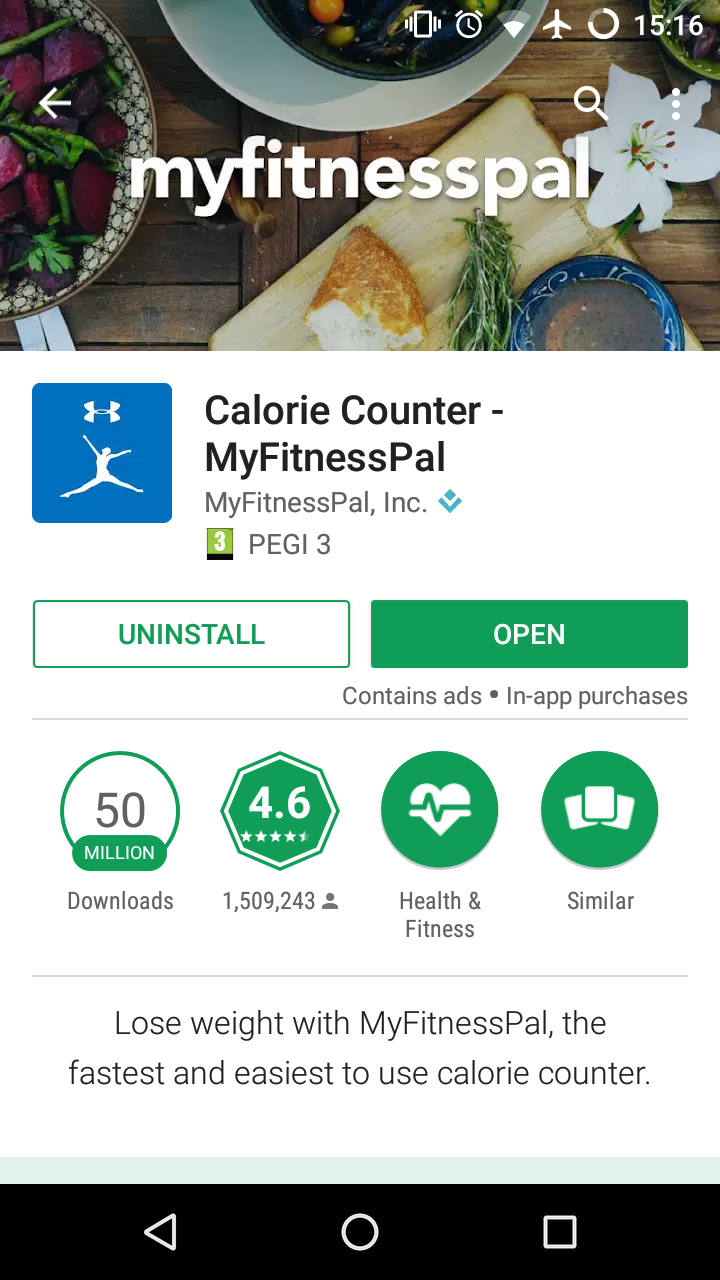
\includegraphics[width=5cm,scale=0.5]{Figures/2/mfp1.png}
\caption{Google Play Store page of MyFitnessPal App}
\label{fig:mfp}
\end{figure}

\begin{figure}[ht]
\centering
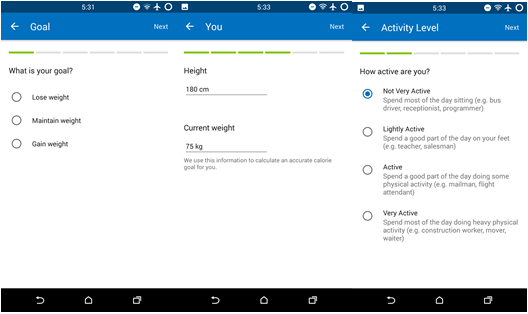
\includegraphics[width=10cm]{Figures/2/mfp2.png}
\caption{Procedure to Create a MyFitnessPal Account}
\label{fig:mfp2}
\end{figure}

\begin{figure}[ht]
\centering
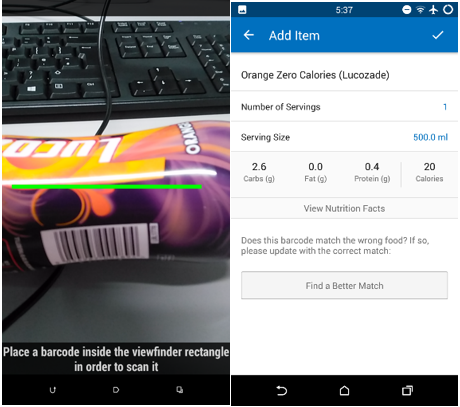
\includegraphics{Figures/2/mfp3.PNG}
\caption{Barcode Scanning with MyFitnessPal}
\label{fig:mfp2}
\end{figure}

The other app tested was Nutracheck. To start using Nutracheck a user is required to create an account. The registration procedure is very similar to MyFitnessPal's. For entering meals, the app also has a barcode scanner and a search function. One advantage of Nutracheck over MyFitnessPal is that it displays images of food in the search results \autoref{fig:eat}. However,  a  barcode scanner of this app recognised fewer barcodes that a barcode scanner in MyFitnessPal when it was tried.

Final app that was tested was Lifesum. It also requires completing a survey, to start using it, and uses a barcode scanner and a search function for adding food. An interesting feature that this app has is a food quality rating. It rates a quality of food according to its nutrition facts and presents the user with a rank of food from A to F \autoref{fig:life}.


\begin{figure}[!tbp]
  \centering
  \begin{minipage}[b]{0.4\textwidth}
    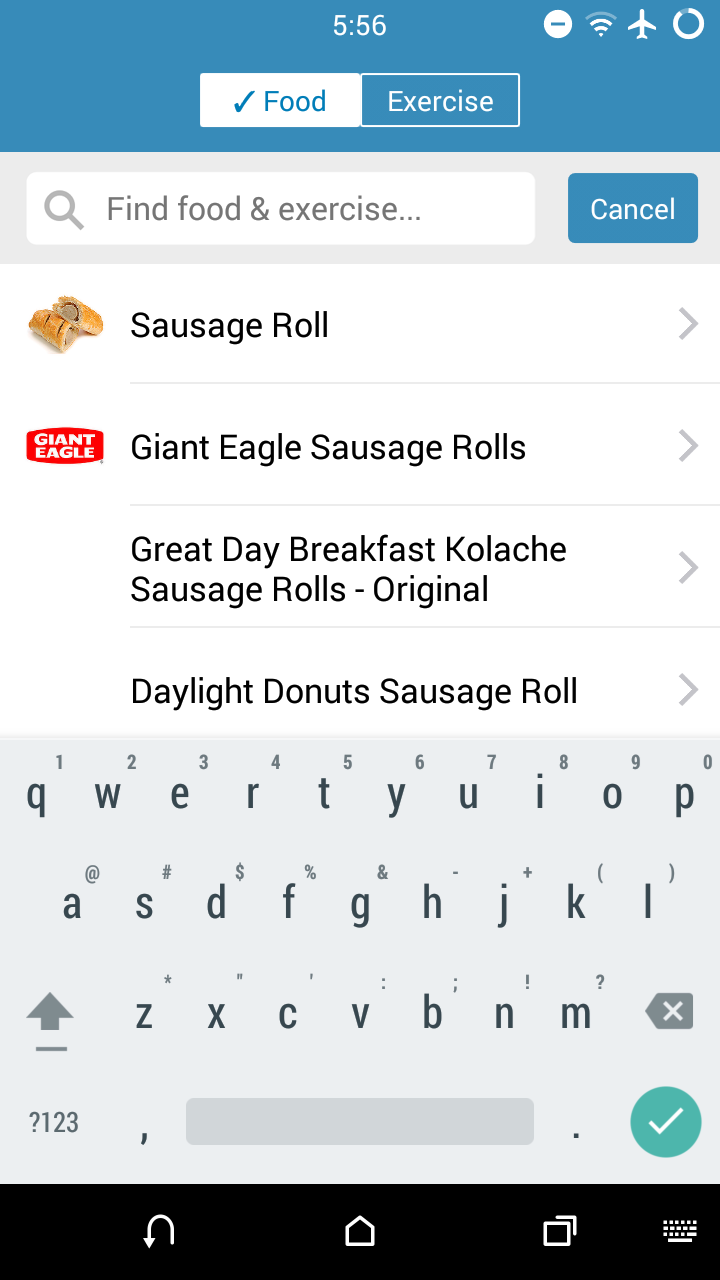
\includegraphics[width=\textwidth]{Figures/2/eat.png}
    \caption{Food  Search in Nutracheck}
    \label{fig:eat}
  \end{minipage}
  \hfill
  \begin{minipage}[b]{0.4\textwidth}
    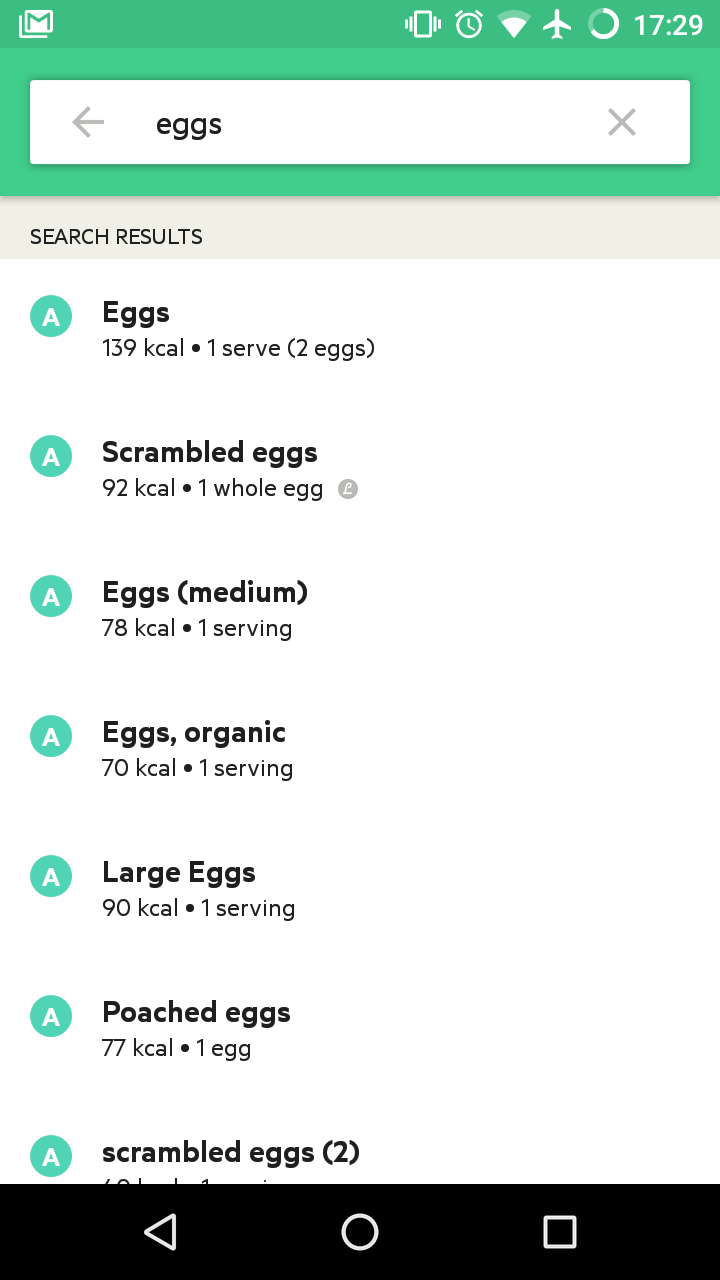
\includegraphics[width=\textwidth]{Figures/2/mm.png}
    \caption{Food  Search in LifeSum}
    \label{fig:life}
  \end{minipage}
\end{figure}


From this short survey, it can be concluded that currently, available calorie counting apps lack innovation. A text-based search and barcode scanners are used as data entry points in all applications. For tracking calorie intake, a user has to enter what he ate manually. The Internet connection is also required to use these applications. Ability to use phone's camera as an input method would significantly improve the usability of the food tracking applications. 

\section{Summary}
In this chapter history of computer vision was reviewed. Then, it was explained why computer vision is such a hard problem. A paper that focused on automatic food image segmentation was summarised and reviewed. Finally, currently available applications for dietary assessment were reviewed. It was concluded, that an automatic food image classifier could extend the capabilities of personal dietary assessment. In the next chapter research methods of the project are discussed.